\begin{frame}{Défis de l'autonomie domiciliaire}
\vspace*{-6.3mm}
\begin{minipage}{.4\linewidth}
\small
Fiabilité de la détection du contexte. 
\\
Multiples axes de variation 
\begin{scriptsize}
(Utilisateurs, domiciles, intervenants).
\end{scriptsize}

Dynamicité.
\end{minipage}
\hfill
\begin{minipage}{.5\linewidth}
    
\includegraphics[scale=0.1]{axe_variation_nill.png}
\end{minipage}
\vfill
% \onslide<2->{
%   \begin{coloredbox}[red]{Problématique}
% \centering
%    Comment couvrir les besoins des services sensibles au contexte?
%   \end{coloredbox}
% }
\end{frame}

\begin{frame}{Défis de l'autonomie domiciliaire}
  \addtocounter{framenumber}{-1}
\vspace*{-6.3mm}
\begin{minipage}{.4\linewidth}
\small
Fiabilité de la détection du contexte. 
\\
Multiples axes de variation 
\begin{scriptsize}
(Utilisateurs, domiciles, intervenants).
\end{scriptsize}

Dynamicité.
\end{minipage}
\hfill
\begin{minipage}{.5\linewidth}
    
\includegraphics[scale=0.1]{axe_variation_1.png}
\end{minipage}
\vfill
% \onslide<2->{
%   \begin{coloredbox}[red]{Problématique}
% \centering
%    Comment couvrir les besoins des services sensibles au contexte?
%   \end{coloredbox}
% }
\end{frame}

\begin{frame}{Défis de l'autonomie domiciliaire}
  \addtocounter{framenumber}{-1}
\vspace*{-6.3mm}
\begin{minipage}{.4\linewidth}
\small
Fiabilité de la détection du contexte. 
\\
Multiples axes de variation 
\begin{scriptsize}
(Utilisateurs, domiciles, intervenants).
\end{scriptsize}

Dynamicité.
\end{minipage}
\hfill
\begin{minipage}{.5\linewidth}
    
\includegraphics[scale=0.1]{axe_variation_2.png}
\end{minipage}
\vfill
% \onslide<2->{
%   \begin{coloredbox}[red]{Problématique}
% \centering
%    Comment couvrir les besoins des services sensibles au contexte?
%   \end{coloredbox}
% }
\end{frame}

\begin{frame}{Défis de l'autonomie domiciliaire}
  \addtocounter{framenumber}{-1}
\vspace*{-6.3mm}
\begin{minipage}{.4\linewidth}
\small
Fiabilité de la détection du contexte. 
\\
Multiples axes de variation 
\begin{scriptsize}
(Utilisateurs, domiciles, intervenants).
\end{scriptsize}

Dynamicité.
\end{minipage}
\hfill
\begin{minipage}{.5\linewidth}
    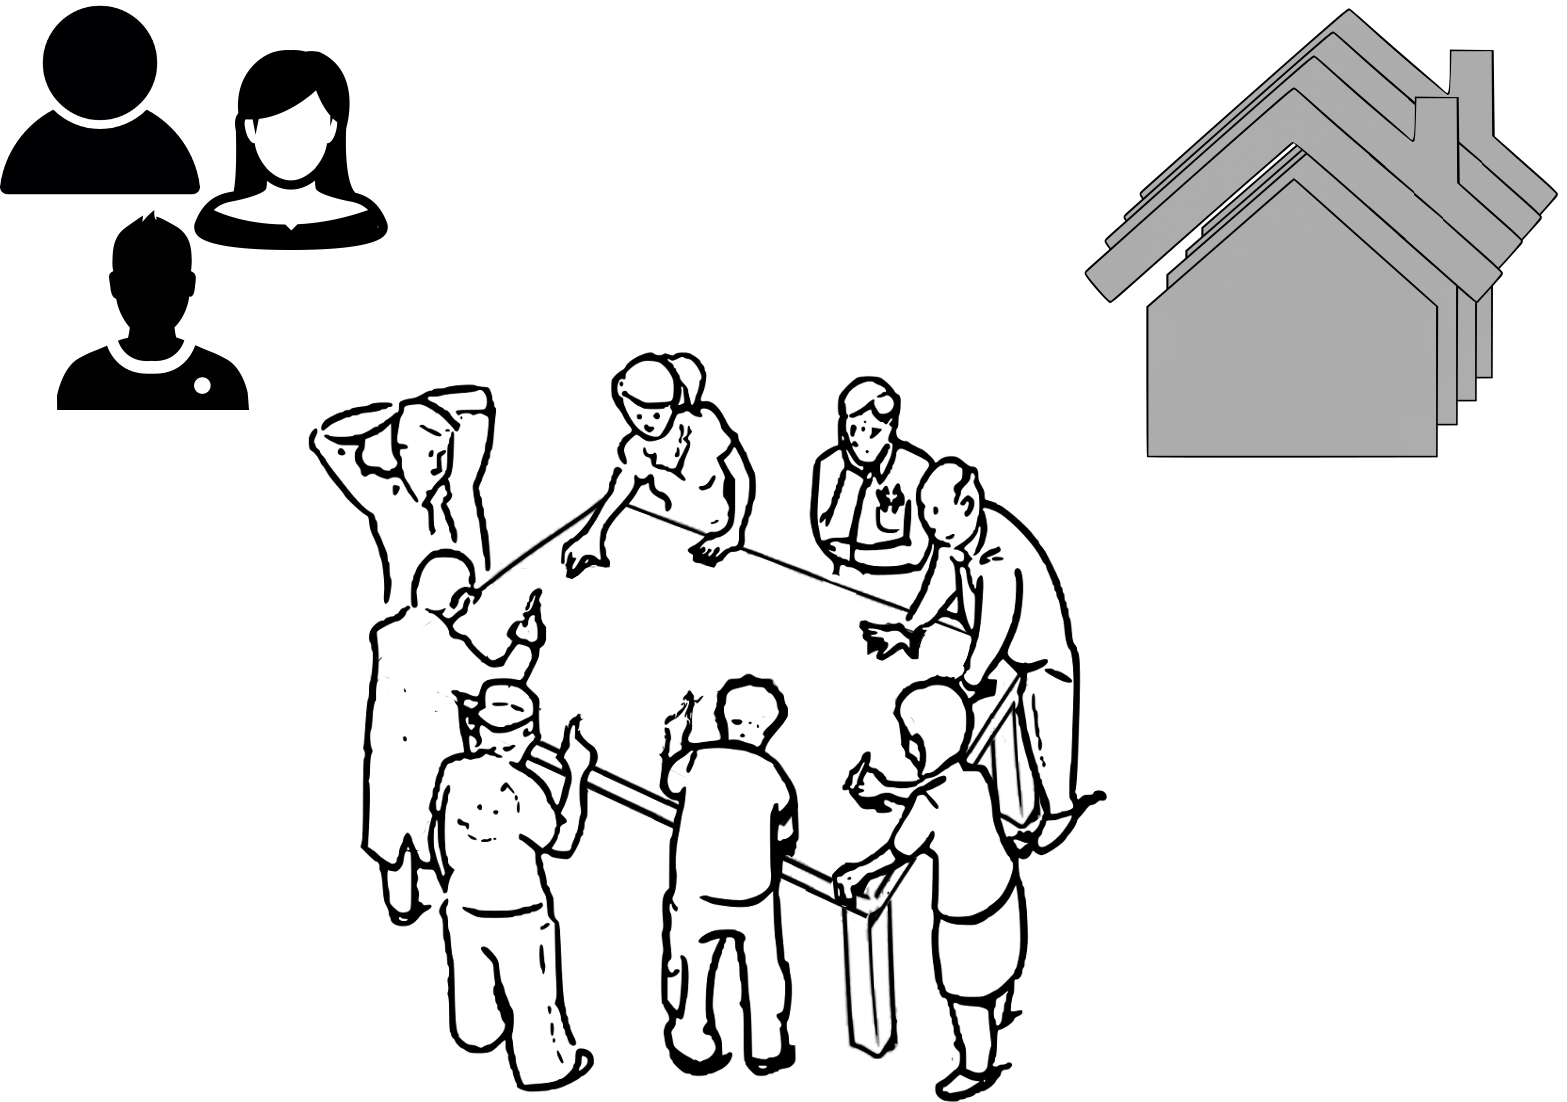
\includegraphics[scale=0.1]{axe_variation_int.png}
\end{minipage}
\vfill
% \onslide<2->{
%   \begin{coloredbox}[red]{Problématique}
% \centering
%    Comment couvrir les besoins des services sensibles au contexte?
%   \end{coloredbox}
% }
\end{frame}

\begin{frame}{Défis de l'autonomie domiciliaire}
  \addtocounter{framenumber}{-1}
\begin{minipage}{.4\linewidth}
\small
Fiabilité de la détection du contexte. 
\\
Multiples axes de variation 
\begin{scriptsize}
(Utilisateurs, domiciles, intervenants).
\end{scriptsize}

Dynamicité.
\end{minipage}
\hfill
\begin{minipage}{.5\linewidth}
    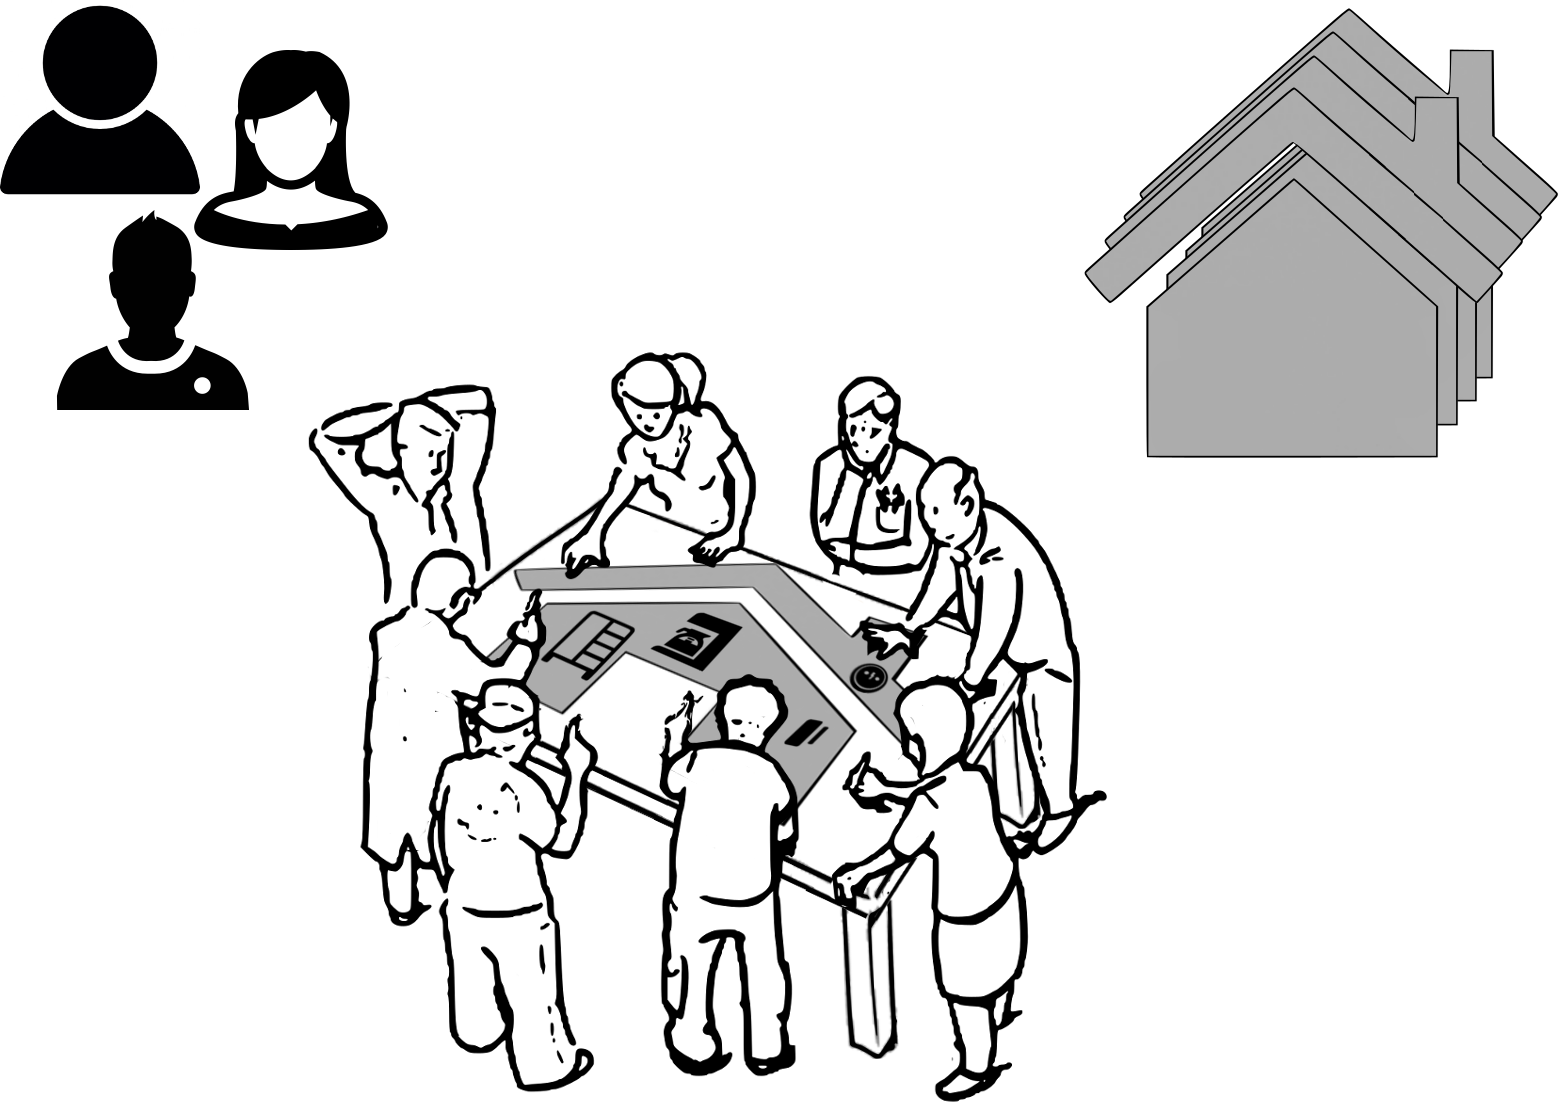
\includegraphics[scale=0.1]{axe_variation_3.png}
\end{minipage}
%\vfill
% \onslide<2->{
%
  \begin{coloredbox}[red]{Problématique}
\centering
   Comment couvrir les besoins des services sensibles au contexte?
  \end{coloredbox}
% }
\end{frame}